\documentclass[letterpaper,notitlepage,twoside]{article}

% Basic imports, increase margins...
\usepackage[margin=0.75in]{geometry}
% Finite State Machine stuff
\usepackage{pgf}
\usepackage{tikz}
\usetikzlibrary{arrows, automata}
% Format tables nicely
\usepackage[latin1]{inputenc}
\usepackage{array}

\usepackage{amsfonts}
\usepackage{amssymb}
\usepackage{amsmath,amsthm}

\renewcommand{\implies}{\Rightarrow} % redefine command "implies"
\renewcommand{\iff}{\Leftrightarrow} % double arrow
\newcommand{\maps}{\rightarrow} % define command "map"
\newcommand{\union}{\cup}
\newcommand{\intersect}{\cap}
\newcommand{\N}{\mathbb{N}} % natural number
\newcommand{\Q}{\mathbb{Q}} % rational number
\newcommand{\R}{\mathbb{R}} % real number
\newcommand{\Z}{\mathbb{Z}} % integers
\newcommand\tab[1][1cm]{\hspace*{#1}} %\tab command

% Add more packages that you use here...

\begin{document}
\title{Homework 25}
\author{Brian Knotten, Brett Schreiber, Brian Falkenstein}
\maketitle
\subsection*{19}
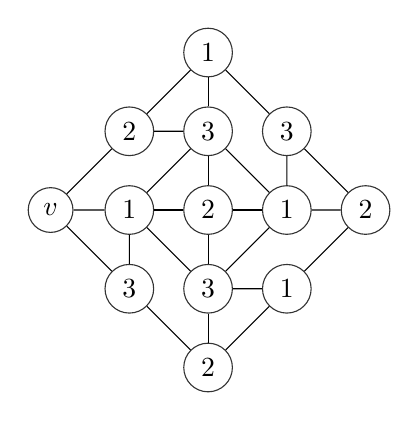
\begin{tikzpicture}
    \node[circle,draw=black!80] (a) at (0, 1) {$v$};
    \node[circle,draw=black!80] (b) at (1, 1) {$1$};
    \node[circle,draw=black!80] (c) at (2, 2) {$3$};
    \node[circle,draw=black!80] (d) at (2, 0) {$3$};
    \node[circle,draw=black!80] (e) at (3, 1) {$1$};
    \node[circle,draw=black!80] (f) at (2, 1) {$2$};
    \node[circle,draw=black!80] (g) at (4, 1) {$2$};
    \node[circle,draw=black!80] (h) at (1, 2) {$2$};
    \node[circle,draw=black!80] (i) at (1, 0) {$3$};
    \node[circle,draw=black!80] (j) at (3, 2) {$3$};
    \node[circle,draw=black!80] (k) at (3, 0) {$1$};
    \node[circle,draw=black!80] (l) at (2, 3) {$1$};
    \node[circle,draw=black!80] (m) at (2, -1) {$2$};
    \draw (a) -- (b) -- (c) -- (e) -- (g);
    \draw (b) -- (d) -- (e);
    \draw (b) -- (f) -- (e);
    \draw (c) -- (f) -- (d);
    \draw (a) -- (h) -- (c);
    \draw (a) -- (i) -- (b);
    \draw (h) -- (l) -- (j) -- (e);
    \draw (l) -- (c);
    \draw (j) -- (g);
    \draw (d) -- (k) -- (g);
    \draw (i) -- (m) -- (k);
    \draw (d) -- (m);
\end{tikzpicture}

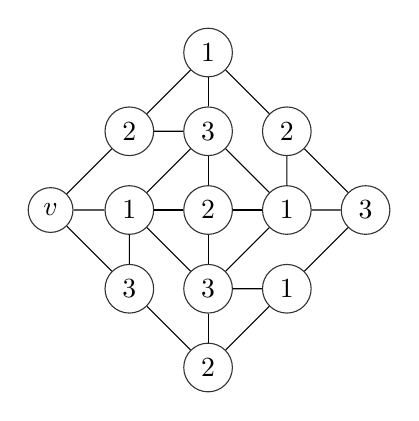
\begin{tikzpicture}
    \node[circle,draw=black!80] (a) at (0, 1) {$v$};
    \node[circle,draw=black!80] (b) at (1, 1) {$1$};
    \node[circle,draw=black!80] (c) at (2, 2) {$3$};
    \node[circle,draw=black!80] (d) at (2, 0) {$3$};
    \node[circle,draw=black!80] (e) at (3, 1) {$1$};
    \node[circle,draw=black!80] (f) at (2, 1) {$2$};
    \node[circle,draw=black!80] (g) at (4, 1) {$3$};
    \node[circle,draw=black!80] (h) at (1, 2) {$2$};
    \node[circle,draw=black!80] (i) at (1, 0) {$3$};
    \node[circle,draw=black!80] (j) at (3, 2) {$2$};
    \node[circle,draw=black!80] (k) at (3, 0) {$1$};
    \node[circle,draw=black!80] (l) at (2, 3) {$1$};
    \node[circle,draw=black!80] (m) at (2, -1) {$2$};
    \draw (a) -- (b) -- (c) -- (e) -- (g);
    \draw (b) -- (d) -- (e);
    \draw (b) -- (f) -- (e);
    \draw (c) -- (f) -- (d);
    \draw (a) -- (h) -- (c);
    \draw (a) -- (i) -- (b);
    \draw (h) -- (l) -- (j) -- (e);
    \draw (l) -- (c);
    \draw (j) -- (g);
    \draw (d) -- (k) -- (g);
    \draw (i) -- (m) -- (k);
    \draw (d) -- (m);
\end{tikzpicture}


\subsection*{21}
Define the problem described as VDP (vertex disjoint paths). In order to show that $3SAT \leq _{poly} VDP$, we will first show that $VDP$ is self reducible. That is, given the decision problem for VDP, we can determine the paths connecting each $(s_i, t_i)$. \\\\
$VDP_{opt} \leq _{poly} VDP_{decision}$\\

\end{document}
